


%%%%%%% GPUs: Disillusion %%%%%%%

\begin{frame}{100x Speed-Up?}
 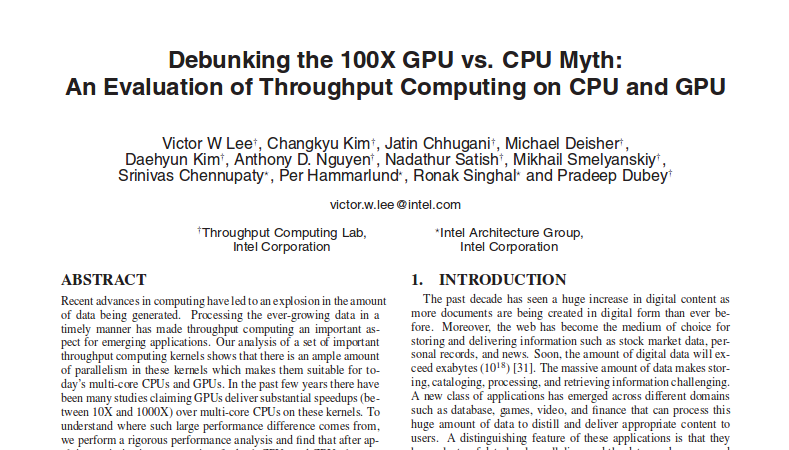
\includegraphics[width=\textwidth]{figures/debunking-100x}
 \begin{center} \vspace*{0.5cm} \small Proc.~ISCA 2010 \end{center}
\end{frame}


\begin{frame}{100x Speed-Up?}
 \begin{center} 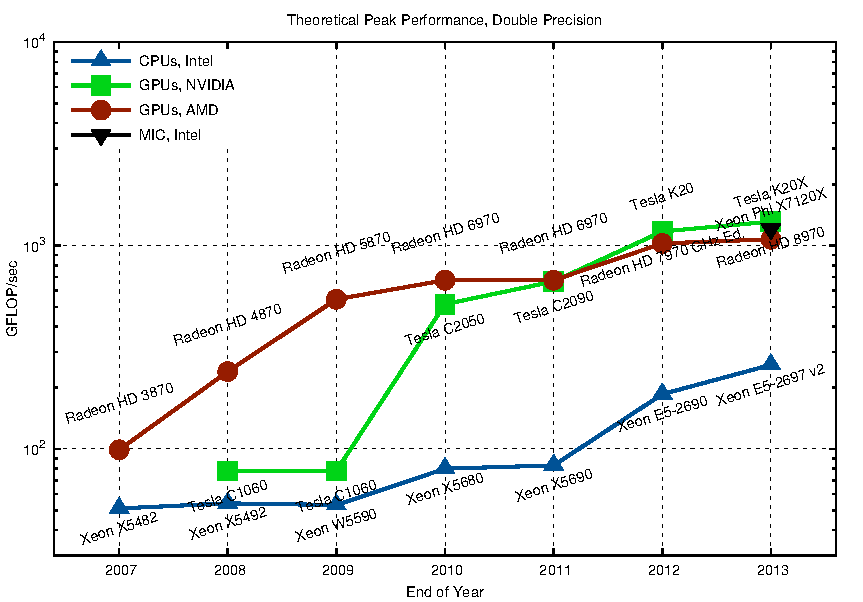
\includegraphics[width=0.95\textwidth]{figures/gflops-dp} \end{center}
\end{frame}

\begin{frame}{100x Speed-Up?}
 \begin{center} 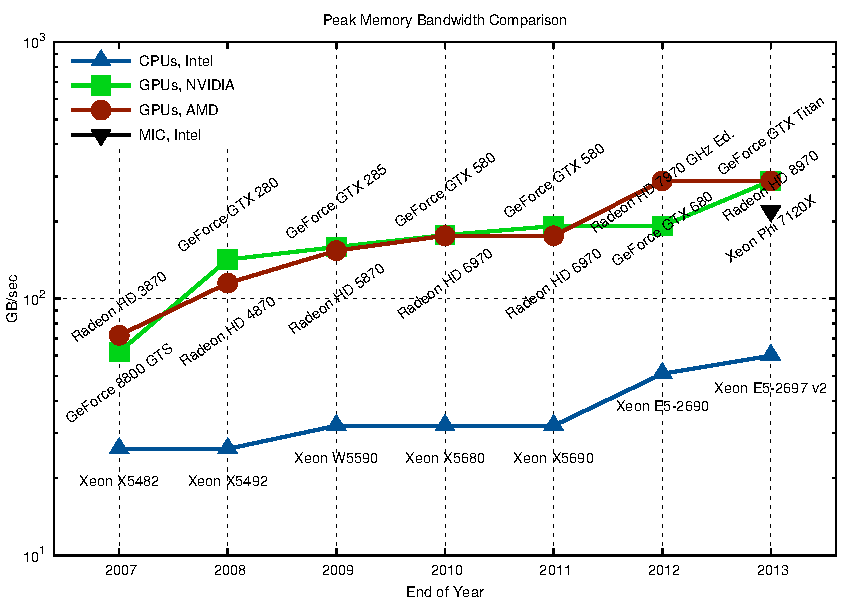
\includegraphics[width=0.95\textwidth]{figures/mem-bw} \end{center}
\end{frame}

\begin{frame}{100x Speed-Up?}
 \begin{center} 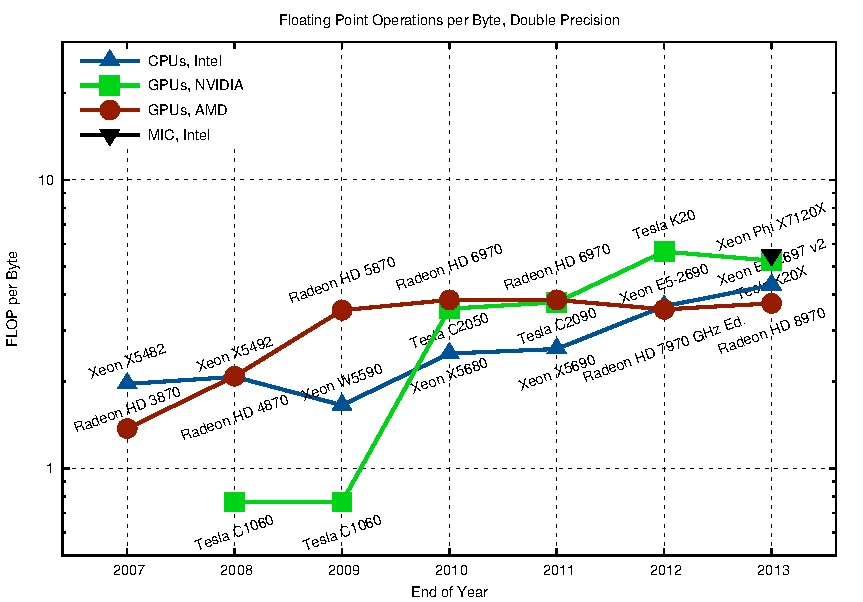
\includegraphics[width=0.95\textwidth]{figures/flop-per-byte-dp} \end{center}
\end{frame}




\begin{frame}[fragile]
\frametitle{GPUs: Disillusion}
 \begin{block}{Computing Architecture Schematic}
  \begin{center}
   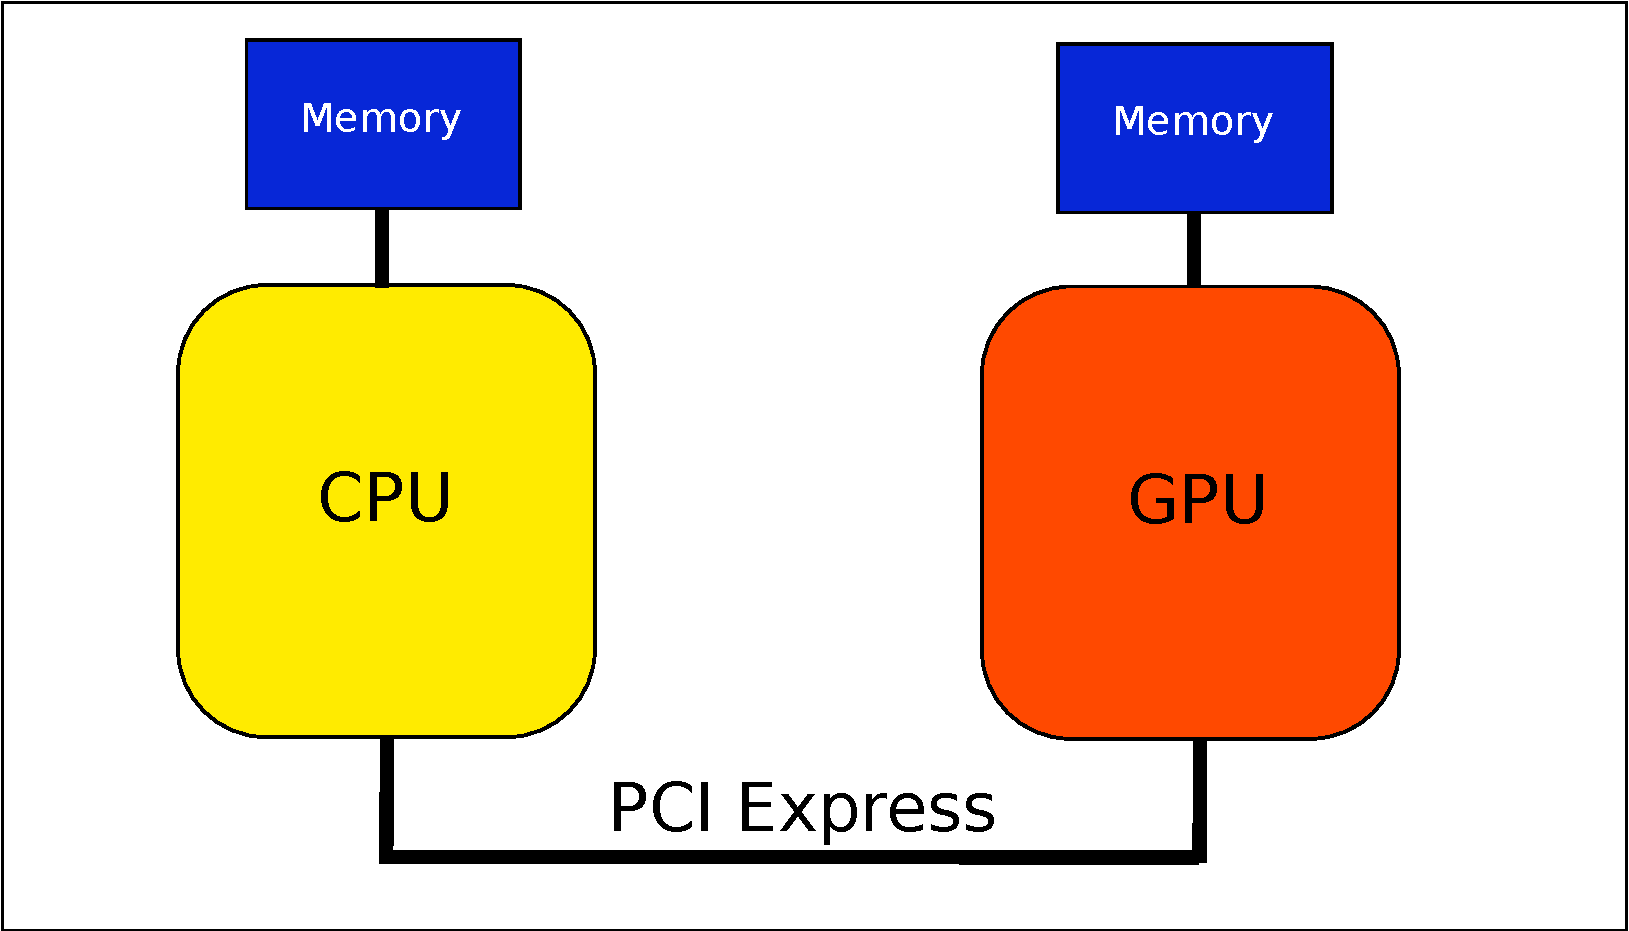
\includegraphics[width=0.8\textwidth]{figures/cpu-gpu-coarse.pdf}
  \end{center}

 
 \begin{itemize}
  \item \vspace*{1.03cm}
 \end{itemize}
 \end{block}

\end{frame}

\begin{frame}[fragile]
\frametitle{GPUs: Disillusion}
 \begin{block}{Computing Architecture Schematic}
  \begin{center}
   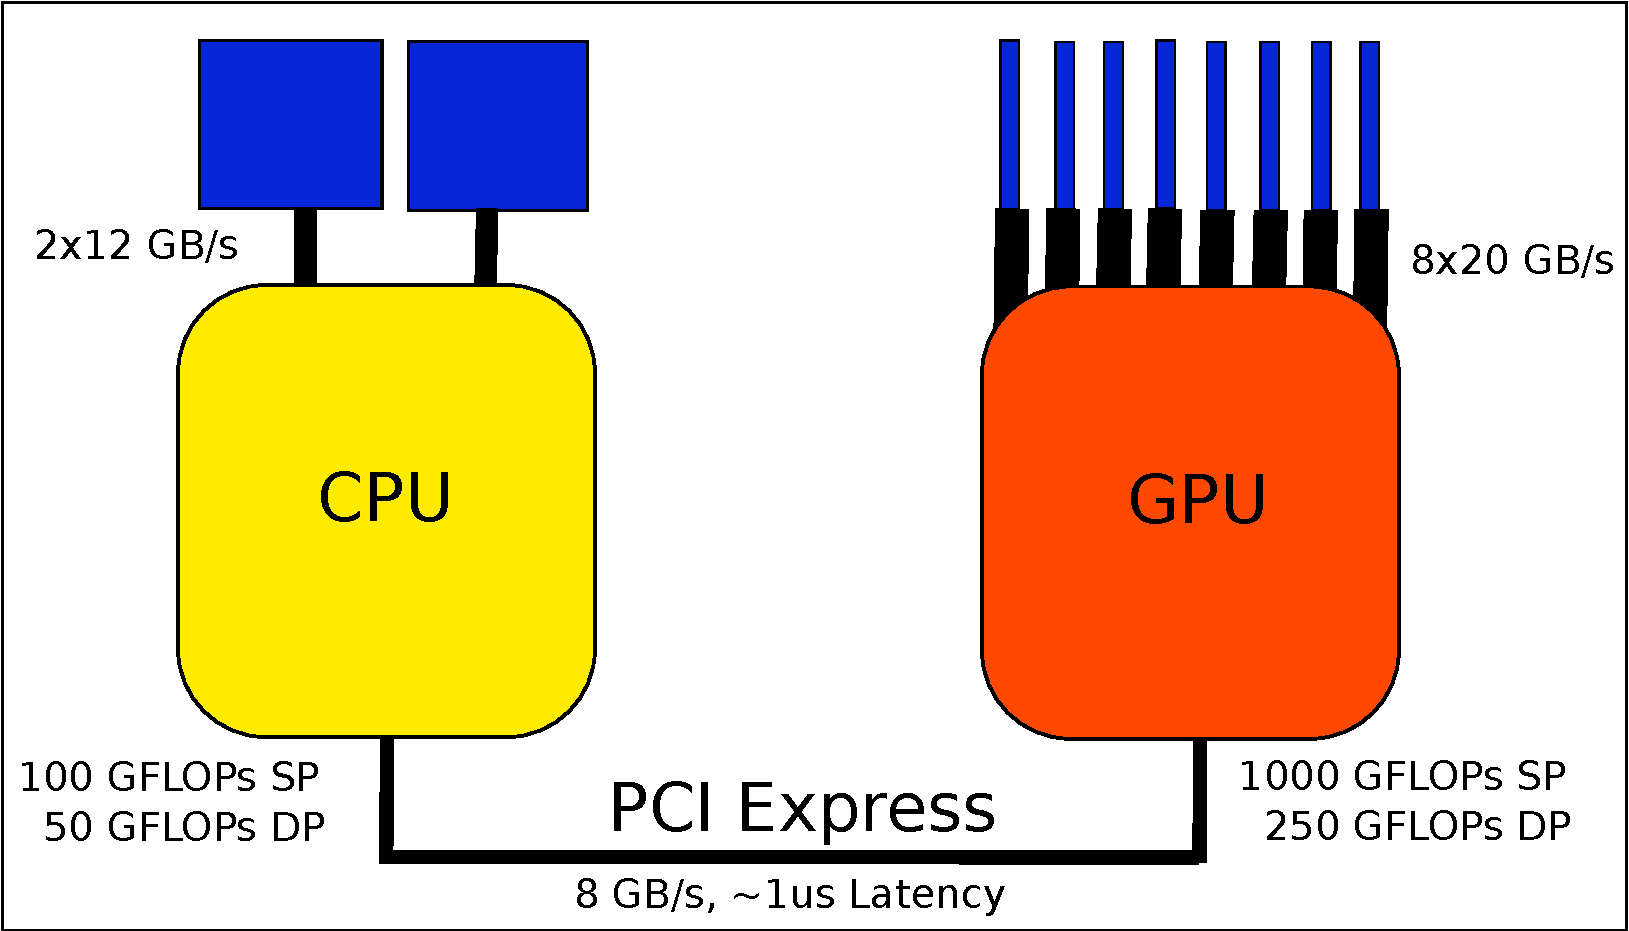
\includegraphics[width=0.8\textwidth]{figures/cpu-gpu-detail.pdf}
  \end{center}

 \begin{itemize}
  \item Good for large FLOP-intensive tasks, high memory bandwidth
  \item PCI-Express can be a bottleneck
  \item $\gg 10$-fold speedups (usually) not backed by hardware
 \end{itemize}
 \end{block}

\end{frame}

